\documentclass[xcolor=pdftex,dvipsnames,table]{beamer}
%
% Choose how your presentation looks.
%
% For more themes, color themes and font themes, see:
% http://deic.uab.es/~iblanes/beamer_gallery/index_by_theme.html
%
\mode<presentation>
{
  \usetheme{Madrid}      % or try Darmstadt, Madrid, Warsaw, ...
  \usecolortheme{default} % or try albatross, beaver, crane, ...
  \usefonttheme{default}  % or try serif, structurebold, ...
  \setbeamertemplate{navigation symbols}{}
  \setbeamertemplate{caption}[numbered]
  \setbeamercolor{framesource}{fg=gray}
  \setbeamerfont{framesource}{size=\tiny}
} 

\usepackage{amsmath}
\usepackage{comment}
\usepackage{geometry}
\usepackage{wrapfig}
\usepackage[english]{babel}
\usepackage[utf8x]{inputenc}
\usepackage[absolute,overlay]{textpos}

\newcommand{\source}[1]{\begin{textblock*}{4cm}(8.7cm,8.6cm)
    \begin{beamercolorbox}[ht=0.5cm,right]{framesource}
        \usebeamerfont{framesource}\usebeamercolor[fg]{framesource} Source: {#1}
    \end{beamercolorbox}
\end{textblock*}}

\title[Completable Futures]{Completable Futures}
\author{Jacky Xu}
\institute{RBC I\&TS}
\date{March 15, 2017}

\begin{document}

\begin{frame}
  \titlepage
\end{frame}

% Uncomment these lines for an automatically generated outline.
%\begin{frame}{Outline}
%  \tableofcontents
%\end{frame}

%%%%%%%%%%%%%%%%%%%%%%%%%%%%%%%%%%%%%%%%%%%%%%%%%%%%%%%%%%%%%%%%%%%%%%%%%%%%%%%%%%%%%%%%%%
\section{Introduction}

\begin{frame}{What is Chess?}
\end{frame}

\begin{frame}{History of AI in Chess}
\end{frame}


\begin{frame}{History of AI in Chess}
\end{frame}

%%%%%%%%%%%%%%%%%%%%%%%%%%%%%%%%%%%%%%%%%%%%%%%%%%%%%%%%%%%%%%%%%%%%%%%%%%%%%%%%%%%%%%%%%%
\section{Board Representation}

\begin{frame}{Board Representation}
\end{frame}

\begin{frame}{Bitboards}
\end{frame}

%%%%%%%%%%%%%%%%%%%%%%%%%%%%%%%%%%%%%%%%%%%%%%%%%%%%%%%%%%%%%%%%%%%%%%%%%%%%%%%%%%%%%%%%%%
\section{Move Generation}

\begin{frame}{Move Generation}
\end{frame}

\begin{frame}[fragile]{Move Generation}
\end{frame}

%%%%%%%%%%%%%%%%%%%%%%%%%%%%%%%%%%%%%%%%%%%%%%%%%%%%%%%%%%%%%%%%%%%%%%%%%%%%%%%%%%%%%%%%%%
\section{Recap and Conclusion}

\begin{frame}{Summary: Components of a Chess Engine}
\end{frame}

\begin{frame}{Future of Chess AI}
\end{frame}

\end{document}

\section{Some \LaTeX{} Examples}

\subsection{Tables and Figures}

\begin{frame}{Tables and Figures}
\begin{itemize}
\item Use \texttt{tabular} for basic tables --- see Table~\ref{tab:widgets}, for example.
\item You can upload a figure (JPEG, PNG or PDF) using the files menu. 
\item To include it in your document, use the \texttt{includegraphics} command (see the comment below in the source code).
\end{itemize}
% Commands to include a figure:
%\begin{figure}
%\includegraphics[width=\textwidth]{your-figure's-file-name}
%\caption{\label{fig:your-figure}Caption goes here.}
%\end{figure}
\begin{table}
\centering
\begin{tabular}{l|r}
Item & Quantity \\\hline
Widgets & 42 \\
Gadgets & 13
\end{tabular}
\caption{\label{tab:widgets}An example table.}
\end{table}
\end{frame}

\subsection{Mathematics}

\begin{frame}{Readable Mathematics}
Let $X_1, X_2, \ldots, X_n$ be a sequence of independent and identically distributed random variables with $\text{E}[X_i] = \mu$ and $\text{Var}[X_i] = \sigma^2 < \infty$, and let
$$S_n = \frac{X_1 + X_2 + \cdots + X_n}{n}
      = \frac{1}{n}\sum_{i}^{n} X_i$$
denote their mean. Then as $n$ approaches infinity, the random variables $\sqrt{n}(S_n - \mu)$ converge in distribution to a normal $\mathcal{N}(0, \sigma^2)$.
\end{frame}


\begin{frame}
\frametitle{Famous Composers}
\begin{center}
\rowcolors{1}{RoyalBlue!20}{RoyalBlue!5}
\begin{tabular}{|l|c|}\hline
J.\ S.\ Bach & 1685--1750 \\
W.\ A.\ Mozart & 1756--1791 \\
L.\ Beethoven & 1770--1827 \\
F.\ Chopin & 1810--1849 \\
R.\ Schumann & 1810--1856 \\
B.\ Bartok & 1881--1945 \\ \hline
\end{tabular}
\end{center}
\end{frame}

\begin{frame}
\frametitle{Two Column Output}
\begin{columns}[c]
\column{1.5in}
Practical \TeX\ 2005\\
Practical \TeX\ 2005\\
Practical \TeX\ 2005
\column{1.5in}
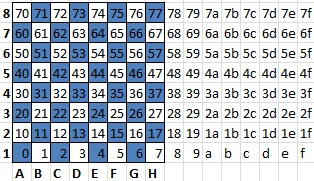
\includegraphics[width=\textwidth,keepaspectratio]{88board.jpg}
\end{columns}
\end{frame}


RESOURCES:

- Beamer tutorial
https://www.tug.org/pracjourn/2005-4/mertz/mertz.pdf

- History of AI in computer chess
http://hightechhistory.com/2011/04/21/a-history-of-computer-chess-%E2%80%93-from-the-mechanical-turk-to-%E2%80%9Cdeep-blue%E2%80%9D/

- Useful timeline of Computer Chess
http://www.thebestschools.org/magazine/brief-history-of-computer-chess/

- (old?) Chess AI Presentation
http://www.cs.bham.ac.uk/~jxb/IAI/w9g.pdf

- How computers play chess
http://www.slideshare.net/carlosjustiniano2/how-computers-play-chess-26552933

- Paper on how Stockfish works
http://rin.io/chess-engine/

- MiniMax Algorithm
http://web.cs.wpi.edu/~rich/courses/imgd4000-d09/lectures/E-MiniMax.pdf

- Diminishing returns on additional search
https://chessprogramming.wikispaces.com/Depth?responseToken=b08a10614bc08c7eb5cf32c8497f34e8#cite_note-7

- Cool Alpha-Beta pruning applet
http://will.thimbleby.net/algorithms/doku.php?id=minimax_search_with_alpha-beta_pruning

- Alpha-Beta pruning and minimax
http://web.cecs.pdx.edu/~mm/AIFall2011/GamePlaying.pdf

CODE EXAMPLES:
\begin{frame}{What is Chess?}
\vskip 1cm
\begin{block}{Examples}
Some examples of commonly used commands and features are included, to help you get started.
\end{block}
\end{frame}
